\documentclass[10pt,twocolumn]{article}
\usepackage[a4paper,margin=0.8in]{geometry}
\usepackage{graphicx,booktabs,amsmath,hyperref,cite,array}
\usepackage[T1]{fontenc}
\title{SafeVoice over Ad-hoc Mesh or Wi-Fi? A Controlled ns-3 Study of Severity-Prioritised SOS Delivery in a Multi-Storey Hostel}
\author{Aryan \\ \small Dept.\ of Electronics and Communication Engineering, Bharati Vidyapeeth College of Engineering, New Delhi\\ \small (draft; co-authors and affiliations to be added)}
\date{}
\begin{document}
\twocolumn[\maketitle
\begin{abstract}
SafeVoice is a campus tool that scores ragging/bullying reports with an NLP pipeline and raises an alert for critical cases. We ask whether alerts should travel over an infrastructure-independent
802.11 ad-hoc mesh (AODV) with severity-based priority, instead of ordinary Wi-Fi. Using ns-3.44 and a 4-floor hostel model, we compare (A) a mesh with EDCA and a push-out severity queue, (B) the same mesh without priority,
(C) provisioned 8-AP infrastructure Wi-Fi, and (C-up) infrastructure whose shared uplink is congested, with one workload file shared by all scenarios, load levels calibrated to the mesh's saturation capacity, and
208 executed runs. Provisioned infrastructure delivered 100\% of critical alerts at all loads and outperformed the mesh. Severity priority gave no measurable gain over the plain mesh up to high load and reduced critical delivery at saturation
(68.7\% vs 88.4\%, 8 paired runs; unadjusted $p=0.0078$, not significant after Holm correction); an ablation links the deficit to the EDCA mechanism, whose cause we did not establish.
The mesh did outperform an infrastructure path with a congested uplink at high and saturated load (+14 and +20 pp). We report four simulation artefacts caught by validation gates, the scale-down from our plan, and limits on statistical power.
We conclude that the mesh is a useful fallback path but that the priority scheme as designed is not supported by the evidence.
\end{abstract}\vspace{1em}]
\section{Introduction}
Ragging and cyberbullying remain persistent problems in Indian higher education despite regulation~\cite{ugc2009}.
SafeVoice is a victim-initiated reporting tool: a student pastes a message, a DistilBERT toxicity classifier and a zero-shot
DistilBART context classifier produce a composite severity score in $[0,1]$, LIME explains the decision~\cite{ribeiro2016,sanh2019},
and \emph{critical} cases (score $\ge 0.75$) trigger an immediate counsellor alert.
The NLP pipeline decides \emph{how urgent} a report is; it says nothing about whether the alert \emph{arrives}.
In a hostel the delivery path is the building's Wi-Fi and the Internet uplink behind it, and these are least reliable exactly when many
people are online (nights, exams) or when an incident causes a surge of traffic.

This paper studies the transport layer underneath SafeVoice. We ask three questions:
(Q1) if alerts travel over an infrastructure-independent multi-hop ad-hoc mesh formed by the students' phones, does tagging them with
the NLP severity and prioritising them by severity improve delivery of the most severe alerts compared with the same mesh without priority?
(Q2) how does the mesh compare with a conventional infrastructure Wi-Fi deployment, both when the infrastructure is well provisioned
and when its shared uplink is congested? (Q3) which priority mechanism (802.11e EDCA, a severity-aware queue discipline, or both) is responsible
for any gain, and how do the systems behave under node or access-point failure and during a sudden crisis burst?

\paragraph{Contributions.}
(i) A single, tested mapping from the application's severity score to network classes (DSCP/802.11e access category/queue band).
(ii) An ns-3 study framework with explicit fairness controls: one scenario-independent workload file whose hash is logged per run
(identical positions, mobility, traffic and failures in all scenarios), identical PHY, queue sizes and rate settings, and a push-out
priority queue discipline with a unit test.
(iii) A validation record. Four modelling artefacts that would each have produced misleading results were detected by sanity gates and fixed
(Section~\ref{sec:validation}); we report them because they are easy to reproduce in other ns-3 studies.
(iv) An honest evaluation, including conditions where the proposed design does not help and where infrastructure Wi-Fi is simply better.
All code, workloads and raw per-packet logs are released with the paper.

\section{Background and Related Work}
\textbf{Ad-hoc routing.} AODV~\cite{rfc3561} discovers routes on demand by flooding route requests; its behaviour in dense networks is
dominated by control traffic and by the broadcast-storm effect~\cite{ni1999}. Comparative studies of MANET protocols~\cite{broch1998,das2000}
motivate our choice of a reactive protocol for a mostly static, partly mobile hostel. Link quality matters: shortest-hop routes found over
weak links perform badly~\cite{decouto2003}; we observed exactly this effect (Section~\ref{sec:validation}).
\textbf{Service differentiation.} IEEE 802.11e EDCA gives four access categories (voice, video, best effort, background) different
contention parameters and transmit-opportunity limits~\cite{ieee80211,mangold2003}; the saturation behaviour of the underlying
DCF is analysed in~\cite{bianchi2000}. EDCA differentiates \emph{channel access}; it does not by itself decide which packet is dropped when
a buffer fills, which is why we also evaluate a queue-level mechanism.
\textbf{Simulation validity.} Wireless simulators embed assumptions (propagation, interference, capture) that can change conclusions~\cite{kotz2004};
we therefore state every PHY/propagation assumption and list threats to validity explicitly. We use ns-3~\cite{riley2010}.

\section{System Model}
\subsection{From text severity to network class}
The application computes a severity score $s\in[0,1]$ (50\% model probability, 50\% weighted context flags) and maps it to
CRITICAL ($s\ge0.75$), HIGH ($s\ge0.50$), MODERATE ($s\ge0.25$) or LOW. The network study uses three SOS classes
(Table~\ref{tab:map}); \texttt{tools/severity\_bridge.py} is the single definition of the mapping and a unit test parses the application's
configuration to ensure that the thresholds cannot drift apart.
\begin{table}[t]\centering\caption{Severity-to-network mapping used in scenario A.}\label{tab:map}
\small\begin{tabular}{@{}lcccc@{}}\toprule
App risk level & SOS class & DSCP & 802.11e AC & queue band\\\midrule
CRITICAL ($\ge0.75$) & 3 & CS6 & AC\_VO & 3\\
HIGH ($\ge0.50$) & 2 & CS5 & AC\_VI & 2\\
MODERATE/LOW & 1 & 0 & AC\_BE & 1\\
other traffic & -- & 0 & AC\_BE & 0\\\bottomrule\end{tabular}\end{table}

\subsection{Scenarios}
\textbf{A (proposed)}: 802.11n ad-hoc mesh, AODV, severity priority (EDCA mapping of Table~\ref{tab:map} \emph{and} a severity-aware queue discipline).
\textbf{B (fair baseline)}: identical mesh and routing, no priority: all traffic is best effort in a FIFO queue.
\textbf{C (current practice, provisioned)}: infrastructure Wi-Fi: 8 access points (two per floor), each on its own orthogonal 20~MHz channel,
each station statically bound to the AP with the strongest computed signal, APs bridged through a gigabit wired core to a campus server that
hosts the SOS sink; SOS is ordinary best-effort traffic.
\textbf{C-up (current practice, congested uplink)}: as C, but the shared link between the campus core and the server is capacity limited
to $0.3\times$ the mesh saturation capacity, so that it saturates at the same offered load as the mesh (30\% of background flows are gateway-bound).
C-up models the mechanism by which hostel Wi-Fi congests an Internet-dependent alert: a shared bottleneck, not radio capacity.

\section{Simulation Methodology}\label{sec:method}
\subsection{Environment and workload}
All experiments use ns-3.44 (PyPI \texttt{ns3==3.44.post0} libraries; the planned 3.40 source tarball was not reachable from our build
environment) compiled with g++~13.3, C++20, on a 2-vCPU Linux container. The hostel has 4 floors of $40\times15$~m with a central corridor
and 12 rooms per floor (48 rooms). $n$ student phones (default $n=50$; $n\in\{25,75,100\}$ in the sweeps) plus one security desk
(ground-floor corridor) are placed as follows: 80\% of students are static at uniformly random positions in random rooms; 20\% are mobile,
following a random-waypoint model inside their floor's corridor (speed $U(1,1.5)$~m/s, pause $U(0,10)$~s).

\paragraph{Propagation and PHY (identical in A, B, C).} Log-distance path loss (exponent 3.0, 46.68~dB at 1~m) plus a deterministic symmetric
loss of 5~dB per wall and 13~dB per floor slab (a \texttt{PropagationLossModel} subclass: walls are counted analytically along the
straight line; floors from the height difference). 802.11n, 5~GHz, 20~MHz, one spatial stream, fixed HT-MCS3 (26~Mb/s) with
ConstantRate, 16.02~dBm transmit power, receiver sensitivity $-92$~dBm, ns-3's NIST error model, default A-MPDU aggregation. Broadcast frames are sent at the
data MCS. Ad-hoc scenarios share one channel (36); scenario C uses channels 36--64, one per AP.

\paragraph{Queues (identical everywhere).} Every station uses an explicit multi-queue root (\texttt{mq}) with four children of 100 packets,
one per access category (we do not rely on ns-3's default FQ-CoDel), and every Wi-Fi MAC queue is limited to 100 packets and 5~s
lifetime (ns-3's default 500~ms lifetime would silently expire packets and would be mislabelled as congestion). In A the children are
severity push-out queue discs; in B and C they are FIFO.

\paragraph{SOS traffic.} 160-byte UDP datagrams, Poisson arrivals at 3/s network-wide from uniformly random students to the desk; severity 3/2/1 with
probabilities 10/30/60\%; no application retries. At $t=30$~s a crisis burst adds 20 SOS from 20 distinct students within 5~s
(forced mix 5 critical/7 high/8 low). Each packet carries a header with sequence, transmit time, severity and source; all per-packet
statistics are computed from it. The first 10~s are a warm-up (every station pings the desk once so routes/associations exist; excluded
from statistics), followed by a 60~s measurement window (90~s with a failure at $t=50$~s in the robustness experiment); no SOS is generated in
the last 5~s.

\paragraph{Background traffic.} Video-like CBR flows (0.25--0.5~Mb/s, 1200~B) carry 70\% of the offered load and web-like on/off flows
(0.5~Mb/s while ON; ON/OFF exponential with means 1/3~s, 1000~B) 30\%; 30\% of flows go to the gateway (desk or server), the rest to random peers.
Flow rates are scaled down from the video rates in our original plan because a 1--2~Mb/s stream saturates a multi-hop 20~MHz mesh by itself.
\emph{Load levels} are defined as 10/40/80/120\% of the saturation capacity of the ad-hoc mesh, obtained from a calibration sweep
(Section~\ref{sec:calib}).

\subsection{Priority mechanisms}
\emph{EDCA level}: the sender sets the IP ToS from the SOS class (Table~\ref{tab:map}); ns-3 maps DSCP$\gg3$ to the user priority and
hence the access category at every hop, because forwarding preserves the IP header.
\emph{Queue level}: \texttt{SvPriorityQueueDisc} has four severity bands, strict-priority dequeue, FIFO within a band, and \emph{push-out}:
when the disc is full and a strictly lower non-empty band exists, the oldest packet of the lowest non-empty band is dropped and the arrival is accepted;
otherwise the arrival is dropped. (ns-3's \texttt{PrioQueueDisc} does not push out.) The severity is read from the UDP destination port
(7001--7003), independently of the ToS, so the queue mechanism can be evaluated without EDCA. A unit test checks dequeue order and
push-out accounting. Because \texttt{mq} gives each access category its own child, the queue discipline only reorders packets \emph{within} an
access category; in the full design that is class~1 versus background inside AC\_BE. The ablation therefore uses EDCA only (FIFO queues),
queue only (all traffic in AC\_BE, severity from the port) and both.

\subsection{Load calibration}\label{sec:calib}
A pilot (scenario B, $n=50$, run~1, 60~s window) offered 1--12~Mb/s of background traffic and measured delivered background goodput
(Table~\ref{tab:calib}); the maximum, 6.48~Mb/s, is taken as the saturation capacity, giving Low/Medium/High/Saturated $=$
0.65/2.59/5.18/7.77~Mb/s offered. The uplink of C-up is $0.3\times6.48=1.94$~Mb/s.
\begin{table}[t]\centering\caption{Saturation calibration of the 50-node mesh (scenario B, one run per point).}\label{tab:calib}
\resizebox{\columnwidth}{!}{\begin{tabular}{@{}rrrr@{}}\toprule
offered (Mb/s) & carried (Mb/s) & bg goodput (Mb/s) & bg PDR (\%)\\\midrule
1 & 1.04 & 0.97 & 93.0\\
2 & 1.95 & 1.73 & 88.7\\
3 & 2.97 & 2.29 & 77.1\\
4 & 4.30 & 3.15 & 73.4\\
6 & 6.11 & 5.09 & 83.4\\
8 & 8.28 & 6.09 & 73.5\\
10 & 9.76 & 6.48 & 66.3\\
12 & 11.88 & 6.39 & 53.8\\
\bottomrule\end{tabular}}\end{table}

\subsection{Metrics and statistics}
Per severity class: delivery ratio (PDR), mean/median/95th-percentile delay and jitter (mean absolute difference of consecutive delays) of \emph{delivered} packets,
and deadline success (fraction of \emph{sent} packets delivered within 2~s or 5~s; undelivered counts as a failure). Delay is always read together with PDR. Also: background
goodput (to detect starvation), AODV control packets/s, drops by cause (queue-disc overflow, push-out, MAC queue expiry, MAC retry limit,
no route), hop count of delivered packets, and for the burst the PDR and delay of critical packets.
Each configuration is simulated with independent seeds (\texttt{RngRun}) and the \emph{same workload file} in all scenarios, so scenarios are compared
pairwise per seed. We report means with 95\% Student-$t$ confidence intervals over runs, paired two-sided Wilcoxon signed-rank tests (ties/zero differences
handled; if all paired differences are zero the result is reported as ``no difference''), the matched-pairs rank-biserial correlation as effect size,
and Holm correction within each metric family. We make no significance claim without a test.

\subsection{Deviations from the original plan}
Our plan called for 100 nodes, 200~s windows and 30 runs. On the available compute (a loaded 100-node, 70~s mesh run costs about 3 CPU-minutes) the full
grid would take days, so: the default scale is $n=50$ with 8 runs per configuration (6/5/3/3 for ablation/robustness/$n{=}100$/density), 60~s windows, 8 APs instead of 4--6
(Section~\ref{sec:validation}), TCP and DSDV are not evaluated (code paths exist but were not run), the ``priority route discovery'' option is not implemented, and we use ns-3.44.
With 8 runs and about 23 critical packets per run the study can detect large effects only; Section~\ref{sec:threats} discusses this.

\section{Validation: gates and the artefacts they caught}\label{sec:validation}
We defined sanity gates before running experiments. They passed only after fixing four problems, each of which would have produced a wrong conclusion:
\begin{enumerate}
\item \textbf{Route-reply storm.} With ns-3's AODV defaults the 100-node mesh generated runaway control traffic even at zero background load (about 4\,000 control packets/s; RREQ/RREP/RERR/HELLO counts 8372/7965/2071/4737 in the pilot), about 4 minutes of wall time per 30~s of simulated time, and only 59--83\% of warm-up pings arrived. Setting the RFC~3561 ``destination only'' flag (no replies from intermediate caches) reduced the counts to 1777/35/134/246 in the 18~s check run, cut wall time about 10$\times$ (91.5~s to 9.0~s for the same run) and raised warm-up delivery to 97--98\%.
\item \textbf{Gray zone.} Route discovery broadcasts used the basic rate, so AODV selected links that fixed-MCS3 unicast could not sustain:
zero-load SOS delivery was 87.2\% (MCS3 unicast, basic-rate broadcast; $n=100$, run~1) versus 97.2\% when broadcasts are sent at the data MCS (98.9\% with MCS0 everywhere).
\item \textbf{Coverage hole.} With one AP per floor, 7 of 100 stations never associated (best-AP signal $-82.4$ to $-84.2$~dBm, below ns-3's $-82$~dBm
preamble-detection threshold), handicapping C at zero load; two APs per floor associate 100/100.
\item \textbf{Wired-backhaul artefact.} Modelling the backhaul as one shared 5~ms CSMA bus capped the wired side at about $1/5\,\text{ms}=200$ frames/s because ns-3's channel is
busy for the whole propagation delay: at 4.3~Mb/s offered ($n=50$) scenario C delivered only 2.12~Mb/s with 51.8\% SOS delivery and \emph{no} wireless drops. A switched star
of full-rate links delivers 100\%. This would have wrongly shown infrastructure Wi-Fi collapsing under load.
\end{enumerate}
Remaining gates (results on the final configuration, $n=50$, 3 runs, zero background load, 60~s): (G3) SOS delivery 96.7--97.7\% in the mesh
and 100\% in C; A, B, and the EDCA-only/queue-only variants differ by at most 1 percentage point (about 2 packets in 190), as expected when nothing is congested;
(G4) the workload hash is identical for A, B, C in every run; (G5) 49.7 of 50 warm-up pings reach the desk before measurement starts and 50/50 stations are associated in C;
(G6) delivered SOS take 1--5 hops (mean 2.3), i.e.\ the mesh is genuinely multi-hop; (G7) the queue-disc unit test passes (13/13 checks) and, with priority on,
critical packets are \emph{relayed} through AC\_VO queues at intermediate nodes (28 relayed versus 23 originated in run~1), so the marking survives forwarding.

\section{Results}\label{sec:results}
All numbers below are produced by \texttt{tools/analyze.py} from the 208 executed runs (main 128, ablation 24, robustness 20, $n{=}100$ 12, density 24);
confidence intervals are 95\% Student-$t$ over runs. About 195 SOS packets are generated per run, of which about 24 are critical (including 5 in the burst), so each per-run critical PDR is a ratio of about 24 packets and has a granularity of about 4 pp; we therefore also report all-SOS delivery.

\subsection{Main comparison ($n=50$)}
Table~\ref{tab:main} and Fig.~\ref{fig:pdr} give the central result.
\begin{table*}[t]\centering\caption{Main grid, $n=50$, 8 runs per cell. ``crit.'' = severity-3 SOS; the deadline column counts undelivered packets as failures; p95 is over delivered packets only; the burst column is the fraction of the burst's critical SOS delivered (pooled over runs).}\label{tab:main}
\small\begin{tabular}{@{}llrrrrr@{}}\toprule
Load & Sys & crit.\ PDR (\%) & crit.\ $\le$2\,s (\%) & crit.\ p95 (s) & burst crit.\ PDR (\%) & bg goodput (Mb/s)\\\midrule
Low & A & 93.4$\pm$4.4 & 92.6$\pm$4.3 & 0.84 & 95 & 0.60\\
 & B & 95.7$\pm$4.4 & 94.2$\pm$4.1 & 0.51 & 92 & 0.55\\
 & C & 100.0$\pm$0.0 & 100.0$\pm$0.0 & 0.00 & 100 & 0.65\\
 & C-up & 100.0$\pm$0.0 & 100.0$\pm$0.0 & 0.00 & 100 & 0.65\\
\midrule
Medium & A & 92.3$\pm$4.8 & 91.3$\pm$5.0 & 0.58 & 90 & 2.03\\
 & B & 92.5$\pm$5.9 & 90.4$\pm$7.1 & 0.94 & 90 & 2.00\\
 & C & 100.0$\pm$0.0 & 100.0$\pm$0.0 & 0.00 & 100 & 2.57\\
 & C-up & 97.8$\pm$5.1 & 97.8$\pm$5.1 & 0.10 & 98 & 2.55\\
\midrule
High & A & 90.6$\pm$7.4 & 90.6$\pm$7.4 & 0.51 & 82 & 4.03\\
 & B & 87.0$\pm$2.5 & 84.5$\pm$2.7 & 1.01 & 92 & 3.87\\
 & C & 100.0$\pm$0.0 & 100.0$\pm$0.0 & 0.00 & 100 & 5.23\\
 & C-up & 76.3$\pm$13.5 & 76.3$\pm$13.5 & 0.43 & 78 & 4.93\\
\midrule
Saturated & A & 68.7$\pm$5.4 & 65.6$\pm$3.3 & 1.35 & 60 & 5.22\\
 & B & 88.4$\pm$5.7 & 84.1$\pm$5.9 & 1.39 & 82 & 5.47\\
 & C & 100.0$\pm$0.0 & 100.0$\pm$0.0 & 0.00 & 100 & 7.74\\
 & C-up & 48.3$\pm$12.1 & 48.3$\pm$12.1 & 0.50 & 35 & 6.40\\
\bottomrule\end{tabular}\end{table*}
\begin{figure}[t]\centering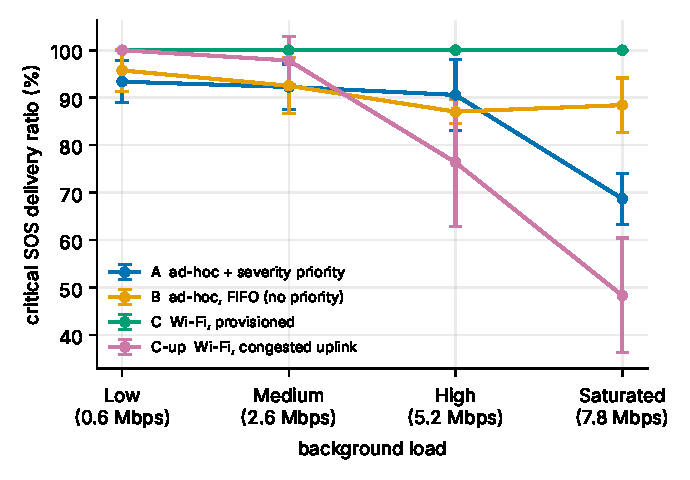
\includegraphics[width=\columnwidth]{figures/fig1_crit_pdr_vs_load.pdf}
\caption{Critical SOS delivery ratio versus background load ($n=50$, mean $\pm$ 95\% CI over 8 runs).}\label{fig:pdr}\end{figure}

\begin{enumerate}
\item \textbf{Provisioned infrastructure Wi-Fi (C) delivered every SOS in every run at every load} (all-SOS PDR 100\%; critical-class p95 delay $\le$1~ms). Under our model, a well-provisioned
multi-AP deployment is simply better than the mesh; the mesh cannot match it.
\item \textbf{The proposed design (A) did not outperform the same mesh without priority (B).} At Low, Medium and High load the difference in critical PDR is
$-2.4$, $-0.2$ and $+3.5$ percentage points (pp), all with $p>0.05$ (Table~\ref{tab:paired}). \textbf{At Saturated load A was worse than B by 19.7~pp}
(68.7\% vs 88.4\%; every one of 8 paired runs favoured B; unadjusted $p=0.0078$, which is the smallest value attainable with 8 pairs; Holm-adjusted $p=0.17$).
With so few pairs we cannot claim a statistically established effect after correction, but the sign is consistent and the effect size large (rank-biserial $r=-1.0$).
\item \textbf{The infrastructure with a congested uplink (C-up) fails first.} It matches or beats the mesh at Low/Medium load but delivers only 76\% of critical SOS at High
and 48\% at Saturated. Against C-up, A is $+14.2$~pp at High ($p=0.16$, not significant) and $+20.4$~pp at Saturated (unadjusted $p=0.0078$, Holm $p=0.17$). C-up's
bottleneck is a modelling choice (uplink $=0.3\times$ the mesh capacity), so this comparison shows \emph{when} a shared uplink hurts, not how often it does.
\item \textbf{Priority does not starve background traffic.} Background goodput in A and B is within 7\% at every load (e.g.\ 4.03 vs 3.87~Mb/s at High; 5.22 vs 5.47~Mb/s at Saturated).
\end{enumerate}
\begin{table}[t]\centering\caption{Paired Wilcoxon tests on critical-class PDR (A minus comparator, same seeds and workloads). $p_{\rm Holm}$: Holm correction over these 12 tests.}\label{tab:paired}
\resizebox{\columnwidth}{!}{\begin{tabular}{@{}llrrrrr@{}}\toprule
Load & A vs & mean diff (pp) & $p$ & $p_{\rm Holm}$ & rank-biserial $r$ & pairs\\\midrule
Low & B & -2.4 & 0.0625 & 0.875 & -0.90 & 8\\
 & C & -6.6 & 0.0078 & 0.172 & -1.00 & 8\\
 & C-up & -6.6 & 0.0078 & 0.172 & -1.00 & 8\\
Medium & B & -0.2 & 0.8438 & 1.000 & -0.14 & 8\\
 & C & -7.7 & 0.0156 & 0.266 & -1.00 & 8\\
 & C-up & -5.6 & 0.0469 & 0.703 & -0.86 & 8\\
High & B & +3.5 & 0.4375 & 1.000 & +0.43 & 8\\
 & C & -9.4 & 0.0312 & 0.500 & -1.00 & 8\\
 & C-up & +14.2 & 0.1562 & 1.000 & +0.71 & 8\\
Saturated & B & -19.7 & 0.0078 & 0.172 & -1.00 & 8\\
 & C & -31.3 & 0.0078 & 0.172 & -1.00 & 8\\
 & C-up & +20.4 & 0.0078 & 0.172 & +1.00 & 8\\
\bottomrule\end{tabular}}\end{table}

\paragraph{Delay.} Delivered packets are fast in every system (median delay $\le$7~ms), but the tail differs: critical p95 delay in the mesh grows to about 1.3--1.4~s at Saturated, while in C it is $\le$1~ms (Table~\ref{tab:main}, Fig.~\ref{fig:cdf}).
Because delay statistics exclude lost packets, the deadline column (2~s) is the relevant combined measure, and it follows the PDR ordering.
\begin{figure}[t]\centering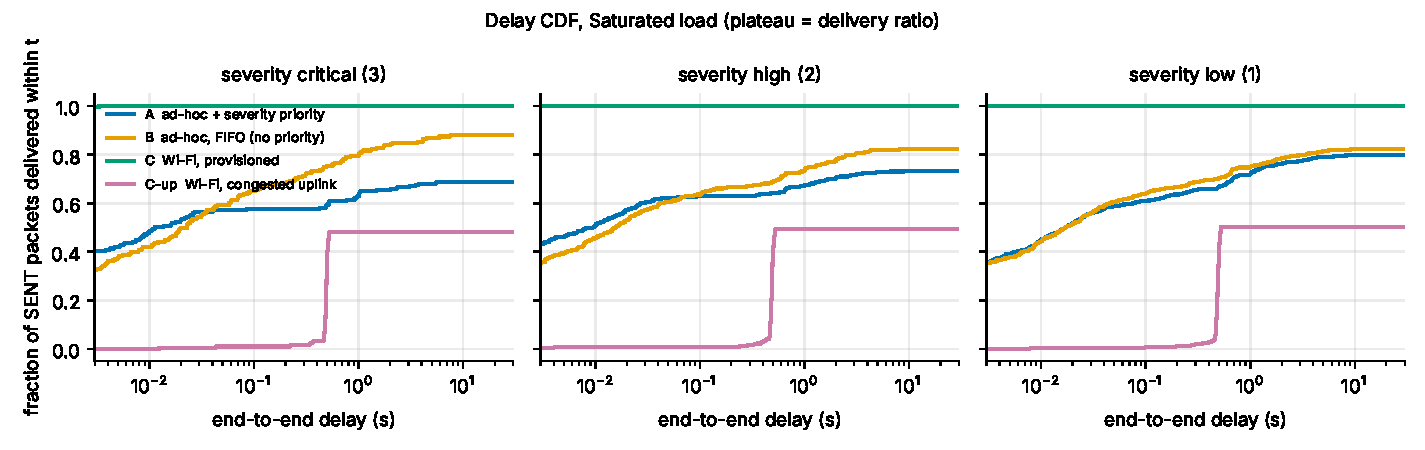
\includegraphics[width=\columnwidth]{figures/fig4_delay_cdf_Saturated.pdf}
\caption{Delay CDFs of delivered SOS per severity at Saturated load (scale of the plateau shows the delivery ratio).}\label{fig:cdf}\end{figure}

\paragraph{Crisis burst.} Fig.~\ref{fig:burst} shows cumulative delivery of the 5 critical SOS in the burst. Ordering is the same as in the steady state (C $>$ B $\ge$ A $>$ C-up at Saturated);
the burst has only 5 critical packets per run (40 over 8 runs), so we draw no further conclusion.
\begin{figure}[t]\centering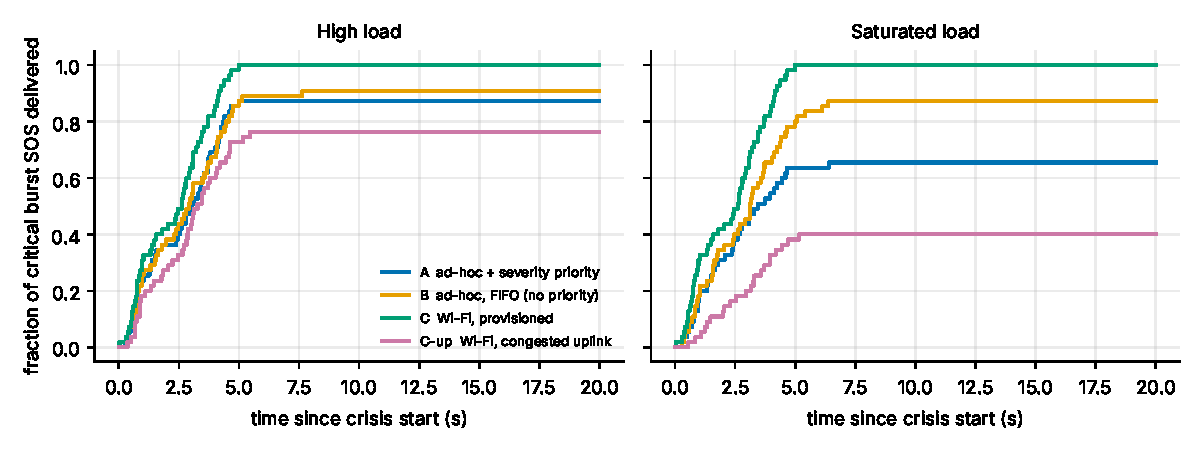
\includegraphics[width=\columnwidth]{figures/fig6_burst_timeline.pdf}
\caption{Cumulative delivery of critical burst SOS after burst start.}\label{fig:burst}\end{figure}

\subsection{Ablation: which priority mechanism?}
Table~\ref{tab:abl} separates the two mechanisms (6 runs; paired tests in \texttt{results/tables/ablation\_paired\_tests.csv}, matched on run number against B).
\begin{table}[t]\centering\caption{Ablation, $n=50$ (B and A rows: 8 runs; ablation rows: 6 runs).}\label{tab:abl}
\resizebox{\columnwidth}{!}{\begin{tabular}{@{}llrrrr@{}}\toprule
Load & Variant & crit.\ PDR (\%) & crit.\ $\le$2\,s (\%) & all-SOS PDR (\%) & push-outs/run\\\midrule
High & B (none) & 87.0$\pm$2.5 & 84.5$\pm$2.7 & 87.1$\pm$4.0 & 0.0\\
 & EDCA only & 86.9$\pm$10.8 & 84.3$\pm$14.9 & 86.9$\pm$5.0 & 0.0\\
 & queue only & 91.2$\pm$3.6 & 88.4$\pm$3.7 & 86.1$\pm$4.6 & 6.7\\
 & both (A) & 90.6$\pm$7.4 & 90.6$\pm$7.4 & 87.7$\pm$4.3 & 2.6\\
\midrule
Saturated & B (none) & 88.4$\pm$5.7 & 84.1$\pm$5.9 & 83.1$\pm$3.3 & 0.0\\
 & EDCA only & 68.3$\pm$13.2 & 67.1$\pm$13.0 & 78.9$\pm$8.0 & 0.0\\
 & queue only & 81.0$\pm$10.1 & 77.5$\pm$12.1 & 83.0$\pm$6.3 & 13.3\\
 & both (A) & 68.7$\pm$5.4 & 65.6$\pm$3.3 & 76.6$\pm$5.4 & 16.9\\
\bottomrule\end{tabular}}\end{table}
At Saturated load the loss relative to B is carried by the EDCA mechanism: EDCA-only $-20.2$~pp ($p=0.031$ unadjusted, 6 pairs), whereas queue-only is $-7.5$~pp ($p=0.19$) and
both together $-19.8$~pp. At High load, queue-only shows the best critical delivery of all variants ($+4.2$~pp over B, $p=0.0625$, which is the closest to significance
reachable with 6 pairs), EDCA-only none ($-0.1$~pp). After Holm correction nothing in the ablation is significant. The queue discipline rarely engages push-out (about 2--17 packets per run), because \texttt{mq} gives each
access category its own queue and only low-priority traffic competes inside AC\_BE.
\emph{We did not isolate why EDCA hurts at saturation.} Candidate explanations that we have \emph{not} tested include more aggressive channel contention
of voice-class transmitters causing more collisions among hidden terminals on a single shared channel, and route-discovery traffic (best effort) being starved by the voice-class data. The data show
that MAC retry-limit drops and no-route events are similar in EDCA-only and B, so a simple rise in retry failures is not the explanation.
\begin{figure}[t]\centering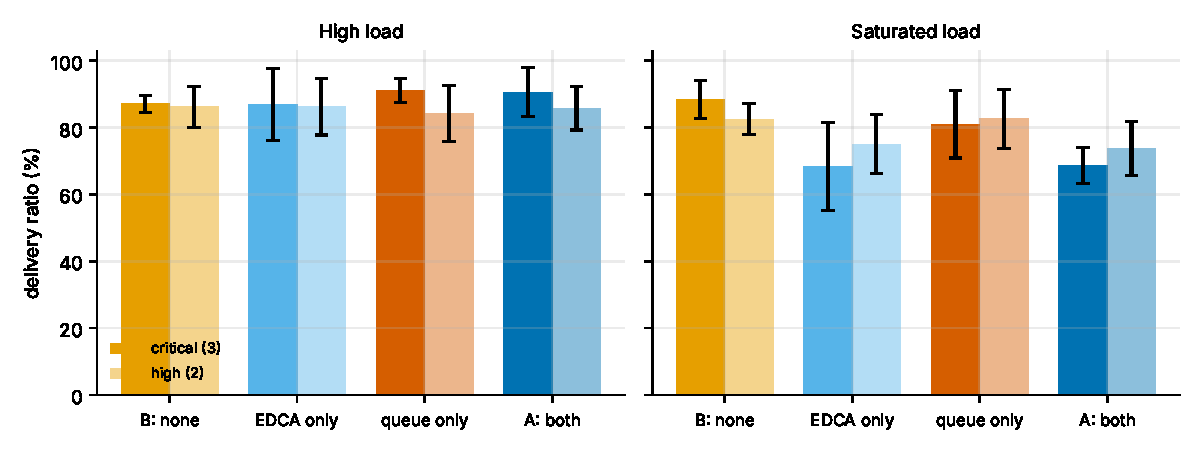
\includegraphics[width=\columnwidth]{figures/fig7_ablation.pdf}
\caption{Ablation of the priority mechanisms.}\label{fig:abl}\end{figure}

\subsection{Scale, density and robustness}
Table~\ref{tab:scale} summarises the sweeps. The $n=25$, 75 and 100 points have only 3 runs each (minimum attainable two-sided exact $p=0.25$), so \emph{no} test is significant and the intervals are wide;
they are included as consistency checks, not as evidence. At $n=100$ the picture is the same as at $n=50$: C 100\%, A below B (75\% vs 86\% critical PDR, 3 runs), and the
congested-uplink variant, which was fixed at the $n=50$ capacity and carries only 30\% gateway-bound background, did \emph{not} saturate in the three $n=100$ runs (100\% critical PDR).
This shows that C-up's collapse depends on how much traffic is gateway-bound and how the uplink is sized, not on the infrastructure as such. AODV control traffic grows with scale from about 340 to 840 packets/s ($n=50$ to 100).
\begin{table*}[t]\centering\caption{Scale and failure experiments at High load. Robustness runs use 90~s windows with the fault at $t=50$~s: 10\% of non-desk nodes switched off in A and B, one AP's radio off in C and C-up with no re-association (a worst-case lower bound for C).}\label{tab:scale}
\small\begin{tabular}{@{}lllrrrr@{}}\toprule
Exp. & $n$ / fault & Sys & runs & crit.\ PDR (\%) & all-SOS PDR (\%) & ctrl pkts/s\\\midrule
density & n=25 & A & 3 & 68.8$\pm$59.3 & 70.8$\pm$19.4 & 170\\
density & n=25 & B & 3 & 64.0$\pm$53.3 & 70.2$\pm$31.2 & 160\\
density & n=25 & C & 3 & 100.0$\pm$0.0 & 100.0$\pm$0.0 & 0\\
density & n=25 & C-up & 3 & 95.7$\pm$18.7 & 97.4$\pm$10.1 & 0\\
\midrule
main & n=50 & A & 8 & 90.6$\pm$7.4 & 87.7$\pm$4.3 & 339\\
main & n=50 & B & 8 & 87.0$\pm$2.5 & 87.1$\pm$4.0 & 347\\
main & n=50 & C & 8 & 100.0$\pm$0.0 & 100.0$\pm$0.0 & 0\\
main & n=50 & C-up & 8 & 76.3$\pm$13.5 & 80.9$\pm$11.2 & 0\\
\midrule
density & n=75 & A & 3 & 80.3$\pm$21.4 & 82.8$\pm$7.6 & 597\\
density & n=75 & B & 3 & 88.9$\pm$33.9 & 87.6$\pm$10.6 & 594\\
density & n=75 & C & 3 & 100.0$\pm$0.0 & 100.0$\pm$0.0 & 0\\
density & n=75 & C-up & 3 & 78.9$\pm$59.9 & 77.8$\pm$61.5 & 0\\
\midrule
confirm & n=100 & A & 3 & 75.1$\pm$18.2 & 85.6$\pm$1.3 & 840\\
confirm & n=100 & B & 3 & 85.8$\pm$2.1 & 87.7$\pm$6.2 & 900\\
confirm & n=100 & C & 3 & 100.0$\pm$0.0 & 100.0$\pm$0.0 & 0\\
confirm & n=100 & C-up & 3 & 100.0$\pm$0.0 & 99.1$\pm$4.0 & 0\\
\midrule
robust & 10\% nodes & A & 5 & 79.6$\pm$7.2 & 83.8$\pm$8.1 & 325\\
robust & 10\% nodes & B & 5 & 85.7$\pm$10.3 & 83.5$\pm$11.8 & 332\\
robust & 1 AP & C & 5 & 94.4$\pm$4.9 & 92.9$\pm$1.7 & 0\\
robust & 1 AP & C-up & 5 & 83.8$\pm$23.2 & 80.2$\pm$22.3 & 0\\
\bottomrule\end{tabular}\end{table*}
Under 10\% node failure A delivers 79.6\% and B 85.7\% of critical SOS over the 90~s window ($p=0.38$, no significant difference). We did not run a fault-free 90~s control, so we do not quantify the loss caused by the failure itself.
With one of 8 APs down, C still delivers 94.4\% (stations bound to the dead AP lose all service because there is no re-association), so its fault tolerance is limited
by static association rather than by the technology. C-up's 83.8\% under AP failure has an interval of $\pm$23 pp and is not distinguishable from the others.

\section{Discussion}
\textbf{Answer to Q1.} In this model, severity priority on the mesh did \emph{not} improve delivery of the most severe alerts. It was neutral up to High load and harmful at Saturated load. We therefore do not claim that the proposed priority scheme works.
\textbf{Answer to Q2.} The mesh is a viable fallback rather than a replacement: it keeps delivering 87--96\% of critical SOS up to High load without any infrastructure, and it beats an infrastructure path whose uplink is the shared bottleneck
(C-up) at High--Saturated load, but a provisioned multi-AP Wi-Fi network outperforms it everywhere. The practical conclusion for SafeVoice is a \emph{dual-path} design: use infrastructure when the uplink is healthy,
and the mesh as an infrastructure-independent fallback when it is not.
\textbf{Answer to Q3.} Of the two priority mechanisms, EDCA is the one associated with the Saturated-load deficit, and the queue discipline alone is neutral to mildly positive; neither is established statistically after correction.
A more promising direction, not implemented here, is prioritising route discovery and control traffic as well as data, because SOS delivery in the mesh is limited by route availability (no-route drops are 1000--1200 per run at Saturated) as well as by queueing.

\section{Threats to Validity and Limitations}\label{sec:threats}
\begin{itemize}
\item \textbf{Simulation versus hardware.} ns-3 abstracts the radio: a deterministic log-distance plus wall/floor loss model (no fading or shadowing), the NIST error model, no interference from outside the building, no device heterogeneity or battery effects. Absolute delivery ratios should not be read as predictions for real phones; the relative ordering is the object of study.
\item \textbf{Statistical power.} The main grid has 8 runs, the ablation 6, robustness 5, scale and density 3, instead of the 30 planned. Each run has only about 24 critical packets, so per-run critical PDR is coarse. The smallest attainable exact two-sided Wilcoxon $p$ is 0.0078 for 8 pairs, which cannot survive Holm correction across 12 tests; we therefore report both unadjusted and adjusted values and make no ``significant'' claims after correction. More runs (or a pooled analysis over all SOS packets) would be needed to resolve the A-versus-B differences.
\item \textbf{Scale-down.} $n=50$ rather than 100 (with $n=100$ checked at one load for 3 runs), 60~s windows instead of 200~s, smaller background flow rates, 8 APs instead of 4--6 (to remove a coverage hole), see Section~\ref{sec:method}. The load levels are tied to the saturation of the 50-node mesh found by a single-run pilot.
\item \textbf{Propagation and mobility.} Walls are counted analytically along the straight line on a regular room grid; mobility is confined to corridors; 80\% of nodes are static. Different building geometry would change hop counts (here 1--7, mean about 2.4).
\item \textbf{Single shared channel in the mesh.} The ad-hoc network uses one 20~MHz channel for all nodes whereas C uses eight, a structural advantage of infrastructure; a multi-channel mesh was out of scope.
\item \textbf{Infrastructure model.} C excludes Internet latency and loss (wired links 0.1~ms), has no AP re-association, and its AP failure result is therefore a lower bound. C-up's congestion is imposed by construction ($0.3\times$ capacity uplink), so its crossing point with the mesh is a function of that parameter.
\item \textbf{Traffic.} Synthetic UDP, no TCP, no application retransmission; SOS datagrams are sent once. Real clients would retry, which would raise delivery in all systems.
\item \textbf{Unexplained effect.} Why EDCA lowers critical delivery at saturation is not established (Section~\ref{sec:results}); our explanations are hypotheses.
\item \textbf{Not evaluated.} DSDV, priority route discovery, NetAnim output, delay under TCP. A custom ns-3 loss model and queue disc were validated by tests and gates, not by comparison with measurements.
\end{itemize}

\section{Conclusion}
We built a reproducible ns-3 study of three transports for the SafeVoice SOS alerts, using identical workloads across all scenarios, and found that
(i) provisioned infrastructure Wi-Fi outperformed the mesh at every load; (ii) severity priority on an AODV mesh was neutral up to high load and worse at saturation, so the hypothesis that it helps is not supported; (iii) the mesh does outperform infrastructure whose shared uplink is congested, supporting a dual-path design;
and (iv) validation exposed four modelling artefacts that would each have changed the conclusions. Future work: more runs, 100--200 nodes at full duration, prioritised route discovery, a multi-channel mesh, TCP and application retries, and validation against a hardware testbed.
The code, workloads, raw per-packet logs and scripts are released with this paper.

\section*{Acknowledgements}
The simulation and analysis code and this manuscript draft were produced with the assistance of an AI model (Claude); the authors are responsible for verifying all content.

\begin{thebibliography}{99}
\bibitem{ugc2009} University Grants Commission, \emph{Regulations on Curbing the Menace of Ragging in Higher Educational Institutions}, 2009.
\bibitem{rfc3561} C.~Perkins, E.~Belding-Royer, S.~Das, ``Ad hoc On-Demand Distance Vector (AODV) Routing,'' RFC 3561, 2003.
\bibitem{ieee80211} IEEE Std 802.11-2020, \emph{Wireless LAN Medium Access Control (MAC) and Physical Layer (PHY) Specifications}.
\bibitem{mangold2003} S.~Mangold, S.~Choi, G.~Hiertz, O.~Klein, B.~Walke, ``Analysis of IEEE 802.11e for QoS support in wireless LANs,'' \emph{IEEE Wireless Commun.}, vol.~10, no.~6, 2003.
\bibitem{bianchi2000} G.~Bianchi, ``Performance analysis of the IEEE 802.11 distributed coordination function,'' \emph{IEEE JSAC}, vol.~18, no.~3, 2000.
\bibitem{riley2010} G.~Riley, T.~Henderson, ``The ns-3 network simulator,'' in \emph{Modeling and Tools for Network Simulation}, Springer, 2010.
\bibitem{broch1998} J.~Broch et al., ``A performance comparison of multi-hop wireless ad hoc network routing protocols,'' \emph{ACM MobiCom}, 1998.
\bibitem{ni1999} S.-Y.~Ni, Y.-C.~Tseng, Y.-S.~Chen, J.-P.~Sheu, ``The broadcast storm problem in a mobile ad hoc network,'' \emph{ACM MobiCom}, 1999.
\bibitem{decouto2003} D.~De Couto, D.~Aguayo, J.~Bicket, R.~Morris, ``A high-throughput path metric for multi-hop wireless routing,'' \emph{ACM MobiCom}, 2003.
\bibitem{kotz2004} D.~Kotz, C.~Newport, R.~Gray, J.~Liu, Y.~Yuan, C.~Elliott, ``Experimental evaluation of wireless simulation assumptions,'' \emph{ACM MSWiM}, 2004.
\bibitem{das2000} S.~R.~Das, C.~E.~Perkins, E.~M.~Royer, ``Performance comparison of two on-demand routing protocols for ad hoc networks,'' \emph{IEEE INFOCOM}, 2000.
\bibitem{ribeiro2016} M.~T.~Ribeiro, S.~Singh, C.~Guestrin, ```Why should I trust you?': Explaining the predictions of any classifier,'' \emph{ACM KDD}, 2016.
\bibitem{sanh2019} V.~Sanh, L.~Debut, J.~Chaumond, T.~Wolf, ``DistilBERT, a distilled version of BERT,'' arXiv:1910.01108, 2019.
\bibitem{wilcoxon1945} F.~Wilcoxon, ``Individual comparisons by ranking methods,'' \emph{Biometrics Bulletin}, vol.~1, no.~6, 1945.
\bibitem{holm1979} S.~Holm, ``A simple sequentially rejective multiple test procedure,'' \emph{Scand. J. Statist.}, vol.~6, 1979.
\end{thebibliography}

\end{document}
